%%%%%
%%Title: HiPi+Bus V0.2 Chapter 4 Section 6
%%Creator: Ando Ki
%%CreationDate: April 1992
%%FileName: sec6
%%RelatedFile: ch4
%%%%%
\section{지정 인터럽트}
지정 인터럽트(direct interrupt)란
인터럽트 요청기가 인터럽트를 받을 처리기의 주소를 지정하여 전송하는 것을 의미한다.
일반적으로 지정 인터럽트는 시험 및 고장 진단을 위한 시스템의 제어 (시험, 고장 진단 등), 
에러의 보고 그리고 실시간 응용 등에 사용될 수 있다. \\
지정 인터럽트는 인터럽트 중재가 끝난 바로 다음 주기에서 시작되고, 5 개의 단계 (Phase)로 구성된다.
각 단계는 버스 클럭 주기 동안 수행된다.
5 단계는 중재 주기를 거쳐 사용 허가를 받은 요청기가
인터럽트 처리기의 주소, 요청기의 주소, 인터럽트의 종류 (벡터)를 전송하는 3 단계와
지정된 처리기가 받은 정보에 대한 응답을 준비하고 응답을 보내는 2 단계로 구성된다.
{\tt <}표~\ref{table:dir-int}{\tt >}는 지정 인터럽트의
단계 별 전송되는 정보와 보내는 측과 받는 측 등을 보여주고 있다.
%\documentstyle[a4]{hbook}
%\begin{document}
%
\begin{table}[htbp]
\caption{지정 인터럽트의 단계별 전송 정보}\label{table:dir-int}
   \begin{center}
   \begin{tabular}{|l|l|l|l|} \hline
	phase & transfer information & from & to \\
\hline \hline
	-5 & interrupt class + slot id + id in slot & IR & IR's \\
	-4 & interrupt class + slot id + id in slot & IR & IR's \\
	-3 & interrupt class + slot id + id in slot & IR & IR's \\
	-2 & interrupt class + slot id + id in slot & IR & IR's \\
	-1 & interrupt class + slot id + id in slot & IR & IR's \\ \hline
	0  & interrupt class + destination address  & IR & IH's \\ \hline
	1  & vector type + source address           & IR & IH \\ \hline
	2  & vector                                 & IR & IH \\ \hline
	3  & dummy                                  & -  & - \\ \hline
	4  & acknowledge                            & IH & IR \\ \hline
   \end{tabular}
   \end{center}
\end{table}
%
%\end{document}

그리고 {\tt <}그림~\ref{figure:dir-int}{\tt >}는 실제
인터럽트 버스상에서의 동작을 보이고 있다.
%
\begin{figure}[htb]
    \centerline{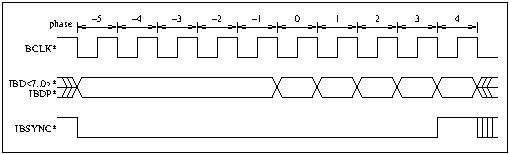
\includegraphics{ch4/FIG/dir-int.jpg}}
   \caption{지정인터럽트의 버스 동작}\label{figure:dir-int}
\end{figure}
%
%
\subsection*{지정 인터럽트 - 단계 -5 --- 단계 -1}
인터럽트 버스를 사용하기에 앞서 수행하는 중재 주기이다.
인터럽트 요청기는 현재 진행 중인 단계가 지정 인터럽트를 보내기에 앞서 수행하는 중재 주기임을
알리기 위해 IBSYNC* 신호를 구동한다.
%
\subsection*{지정 인터럽트 - 단계 0}
이 단계에 전송되는 정보는 종류 정보와 인터럽트를 받는 측(처리기)의 주소가 전송된다.
인터럽트 요청기는 현재 인터럽트 전송이 진행되고 있음을 알리기 위해 IBSYNC* 신호를 구동한다.
비트별 전송 정보는 {\tt <}표~\ref{table:dir-int-p0}{\tt >}과 같다.
%\documentstyle[a4]{hbook}
%\begin{document}
%
\begin{table}[htbp]
\caption{지정 인터럽트 - 단계 0에서 전송되는 정보}\label{table:dir-int-p0}
   \begin{center}
   \begin{tabular}{|l|l|} \hline
	bit field & information \\
\hline \hline
	7, 6 & interrupt class \\ \hline
	5, 4, 3, 2 & slot id \\ \hline
	1, 0 & id in slot \\
\hline
   \end{tabular}
   \end{center}
\end{table}
%
%\end{document}

종류 정보는 지정된 처리기가 저장하게 되는데, 받는 측은 이 값에 따라
다음부터 진행될 단계에 대해서 준비할 수 있게 된다.
종류 필드의 값에 따른 의미는 {\tt <}표~\ref{table:int-class}{\tt >}와 같다. \\
이 단계에서 전송되는 비트 0에서 비트 5까지의 값은 다음 주기부터 전송되는 인터럽트를
받을 처리기의 주소를 나타내는데, 이때 지정된 처리기는 요청기에서 오는 인터럽트 정보를
받고, 해당 동작을 수행하게 된다.
비트 0부터 비트 5까지의 값에 대한 처리기의 할당은 {\tt <}표~\ref{table:ih-ga}{\tt >}과 같다.
Slot ID가 15일 경우는 모든 처리기가 지정된다.
모든 처리기가 지정될 경우, 다음 주기부터 전송되는 정보를 모든 처리기는 동시에 저장하게 된다.
%\documentstyle[a4]{hbook}
%\begin{document}
%
\begin{table}[htbp]
\caption{지정 인터럽트 단계 0의 처리기 어드레스}\label{table:ih-ga}
   \begin{center}
   \begin{tabular}{|l|l|l|} \hline
	Slot ID & ID in Slot & Interrupt Requester \\
\hline \hline
	0 - 12   & x & Slot  0 - Slot 12 \\
	13  - 14 & x & reserved \\
	15 & x & All Handler \\
\hline
   \end{tabular}
   \end{center}
\end{table}
%
%\end{document}

%
\subsection*{지정 인터럽트 - 단계 1}
이 단계에서는 인터럽트 요청기가 처리기에게 벡터의 종류와 자신의 어드레스를 전송한다.
인터럽트 요청기는 현재 인터럽트 전송이 진행 되고 있음을 알리기 위해 IBSYNC* 신호를 구동한다.
처리기의 주소는 6 비트가 사용되고, 상위의 2 비트는 벡터의 종류에 대한 정보를 같이 전송한다.
{\tt <}표~\ref{table:dir-int-p1}{\tt >}는 각 비트별 전송 정보를
나타내고 있다.
%\documentstyle[a4]{hbook}
%\begin{document}
%
\begin{table}[htbp]
\caption{지정 인터럽트 - 단계 1에서 전송되는 정보}\label{table:dir-int-p1}
   \begin{center}
   \begin{tabular}{|l|l|} \hline
	bit field & information \\
\hline \hline
	7, 6 & vector type \\
	5, 4, 3, 2 & slot id \\
	1, 0 & id in slot \\
\hline
   \end{tabular}
   \end{center}
\end{table}
%
%\end{document}

지정 인터럽트에 의해 전송될 수 있는 벡터의 종류는
{\tt <}표~\ref{table:vec-type}{\tt >}과 같다.
모든 형태의 벡터를 전송할 수 있으나, 최대 전송할 수 있는 벡터의 크기가 8 비트로
한정되어 있기 때문에 16 비트의 벡터를 갖는 경우는 하위 8 비트를 0으로 간주한다.
지정 인터럽트에 의해 전송되는 벡터는 주로 E-와 I-Type이 되며,
시스템의 시험이나 진단을 위한 목적으로 사용된다.
E-Type은 마스크가 불가능하기 때문에 도착한 인터럽트는 항상 해당 프로세서로 전달하고,
I-Type의 경우 마스크되어 있으면 도착한 인터럽트를 무시한다.
Q-와 N-Type은 중재 인터럽트와 동일하게 동작한다 (중재 인터럽트 1 참조).
%
\subsection*{지정 인터럽트 - 단계 2}
이 단계에서는 요청기가 처리기로 인터럽트 벡터(Interrupt Vector)를 보낸다.
인터럽트 요청기는 현재 인터럽트 전송이 진행되고 있음을 알리기 위해 IBSYNC* 신호를 구동한다.
인터럽트 벡터는 요청기가 실질적으로 처리기에 원하는 행동이 무엇인지를 담고 있는 것이다.
인터럽트 벡터는 그들이 갖고 있는 의미에 따라 입출력 동작 제어를 위한 것,
각 슬롯에서 발생된 에러의 보고를 위한 것,
각 슬롯에서 보고된 에러의 처리를 위하여 시스템 콘트롤러에서 보내는 제어를 위한 것,
끝으로 프로세서들 사이에 그들이 수행하고 있는 프로세서 제어나 대화를 위한 정보의
교환을 위한 것등으로 분리할 수 있다.
8 비트의 벡터 값에 따른 의미는 \ref{section:vector-type}에서 설명한 바와 같다.
%
\subsection*{지정 인터럽트 - 단계 3}
인터럽트 요청기는 현재 인터럽트 전송이 진행되고 있음을 알리기 위해 IBSYNC* 신호를 구동한다.
인터럽트를 받은 처리기가 요청기에게 응답을 보내기 위해 이제 까지 받은 정보를 점검하여
다음 단계에서 요청기로 보낼 응답을 준비한다.
%
\subsection*{지정 인터럽트 - 단계 4}
인터럽트 요청기는 현재 진행 중인 단계가 지정 인터럽트의 마지막임을 알리기 위해 이제까지
구동하고 있던 IBSYNC* 신호를 걷어낸다.
지정 인터럽트의 최종 단계로, 인터럽트를 받은 처리기가 요청기에게 응답을 보내는 일을 수행한다.
응답 단계에서는 진행된 인터럽트 전송에 에러 발생 여부와 인터럽트 처리기의 상태 등을 전달한다.
{\tt <}표~\ref{table:dir-int-p3}{\tt >}는 전송되는 8 비트의 응답 정보의
각 비트별 의미를 나타내고 있다.
에러가 발생했을 때 해당 비트의 값은 ``거짓''이 된다.
따라서 정확한 순서와 의미로 인터럽트가 전송된 경우는 각 비트의 값이 ``참''이 되도록 하여야만 한다.
%\documentstyle[a4]{hbook}
%\begin{document}
%
\begin{table}[htbp]
\caption{지정 인터럽트 - 단계 3에서 전송되는 정보의 비트별 의미}\label{table:dir-int-p3}
   \begin{center}
   \begin{tabular}{|l|l|} \hline
	bit field & information \\
\hline \hline
	7 & sequence error \\
	6 & parity error \\
	5 & buffer full error \\
	4 & unacceptable error \\
	3 & {\it reserved} \\
	2 & {\it reserved} \\
	1 & {\it reserved} \\
	0 & overwritten error \\
\hline
   \end{tabular}
   \end{center}
\end{table}
%
%\end{document}

\begin{itemize}
	\item 비트 7은 인터럽트 전송 주기 진행에의 에러가 발생했을 경우에 ``거짓''이 되는 비트로
		전송 도중 (DI의 phase4 이나 AI-1의 phase21 제외)에 IBSYNC* 신호가 거짓이
		되었을 경우가 해당된다.
	\item 비트 6은 단계 0, 1 혹은 2에서 전송된 데이터에 패리티 에러가 검출되었을 때 ``거짓''이 된다.
	\item 비트 5는 벡터가 저장될 곳이 다른 인터럽트에 의해 가득찼을 경우에 ``거짓''이 된다.
	\item 비트4는 전송된 벡터를 저장할 수 없는 처리기나 그밖에 정의되지 않은 에러에 의하여
		벡터를 접수할 수 없는 경우에 ``거짓''이 된다.
	\item 비트 0은 처리기에 현재 처리가 지연된 인터럽트(pended interrupt)가 존재했는데 
		새로운 인터럽트가 발생하여 이전 것을 지워지고 새 인터럽트가 저장됐을 경우 ``거짓''이 된다.
\end{itemize}
각 비트는 정의된 상황이 발생했을 경우 ``거짓''이 되도록 함에 따라
처리기가 아무 응답을 안할 경우도 에러로 처리된다. 
또한 두 개 이상의 처리기가 응답을 해야하는 경우(broadcast)에는 한개만이라도 에러가 없다고
응답이 오면 에러가 발생하지 않은 것으로 간주된다.
